\chapter{Projektplan}
\section{Udviklingsproces}
Projektets proces styres efter Unified Process' (UP) principper. Figur \ref{fig:Unified Process} viser udviklingsfaserne i UP.

\begin{figure}[H]
\centering
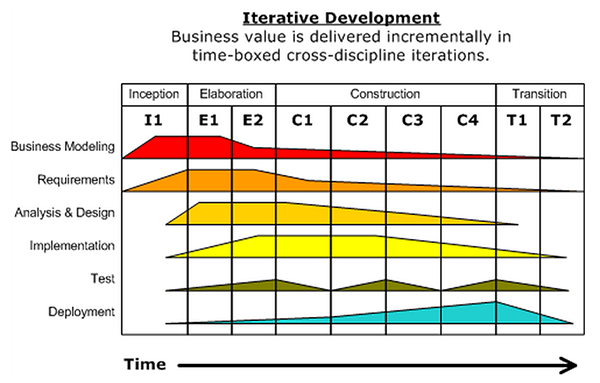
\includegraphics[width=0.6\textwidth]{billeder/up-timetable}
\caption{Unified Process udviklingsforløb}
\label{fig:Unified Process}
\end{figure}

\section{Udviklingsfaser}
\subsection{Inception}
Her blev det fastlagt hvilket projekt, der ønskes udarbejdet, samt overordnede beslutning som platform, delprojekter, eventuel forretnings ide mm. Denne fase er på nuværende tidspunkt overstået.

\subsection{Elaboration}
Denne fase er blevet brugt til test af Estimote Beacons med henblik på at opnå bedre forståelse af produktet og for at definere muligheder og begrænsninger. Det har været et nødvendigt skridt for at kunne udarbejde realistiske krav til produktet. Det var et kritisk skridt da det viste sig at Estimote's specifikationer var anderledes end først antaget, hvilket bevirkede at projektets oprindelige målsætning måtte ændres.  \\

Derudover er alle underprojekter blevet endegyldigt faslagt og ved slutningen af denne fase (før officiel semesterstart d. 27. januar), foreligger foreløbelig kravspecifikation, systemarkitektur og tidsplan. \\

Slutteligt vil byggeserver og testmiljøer til alle underprojekter være konfigureret og klar til brug.

\subsection{Construction}
Når projektet er igang svarer hver konstruktionsfase til et sprint. Foreløbige sprints bliver planlagt på et senere møde inden semesterstart.

\section{Udviklingsprocessser}
I projektet stræber vi efter at få så professionelt et udviklingsmiljø som muligt. Vi har derfor valgt til fulde at benytte os af versionsstyring med GitHub til både kode og dokumentation. Derudover anvender vi Travis-CI til continous integration. Dette passer godt sammen med vores plan om at udvikle testdrevent.
Derudover vil vi benytte os af pair-programming hvor det giver mening.
For at have et samlet overblik over projektets fremgang vil vi anvende Flowdock.